\begin{frame}{Problem: OverFitting in a Neural Network}
	\begin{itemize}
		\item Why does overfitting happen in a neural network?
		\begin{itemize}
			\item There are \tc{keywords}{Too many free parameters}.
		\end{itemize}
	\end{itemize}
    \begin{figure}[H]
        \centering
        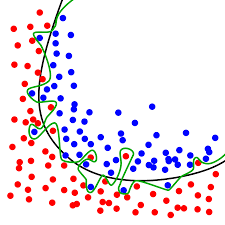
\includegraphics[width=0.4\textwidth]{Figs/section_4/overfitting.png}
        \caption{OverFitting in a neural network, \href{https://en.wikipedia.org/wiki/Overfitting}{Source}}
    \end{figure}
\end{frame}

\begin{frame}{Solution 1: L1/L2 Regularization}
    \begin{itemize}
        \item It is like a linear regression regularizer.
        \item Sum the regularizer term for every \tc{keywords}{layer weight}!
    \end{itemize}
    \begin{columns}
    	\begin{column}[c]{0.5\textwidth}
    			\begin{align*}
    				\scalebox{1.5}{$L = \frac{1}{N} \sum_{i=1}^{N} L(\phi(x_i), y_i)$} \\
    			\scalebox{1.5}{$+ \lambda \sum_{i,j,k} R(W_{j,k}^{(i)})$}
	    		\end{align*}
    	\end{column}
    	\begin{column}[c]{0.5\textwidth}
    		\begin{figure}[H]
    			\centering
    			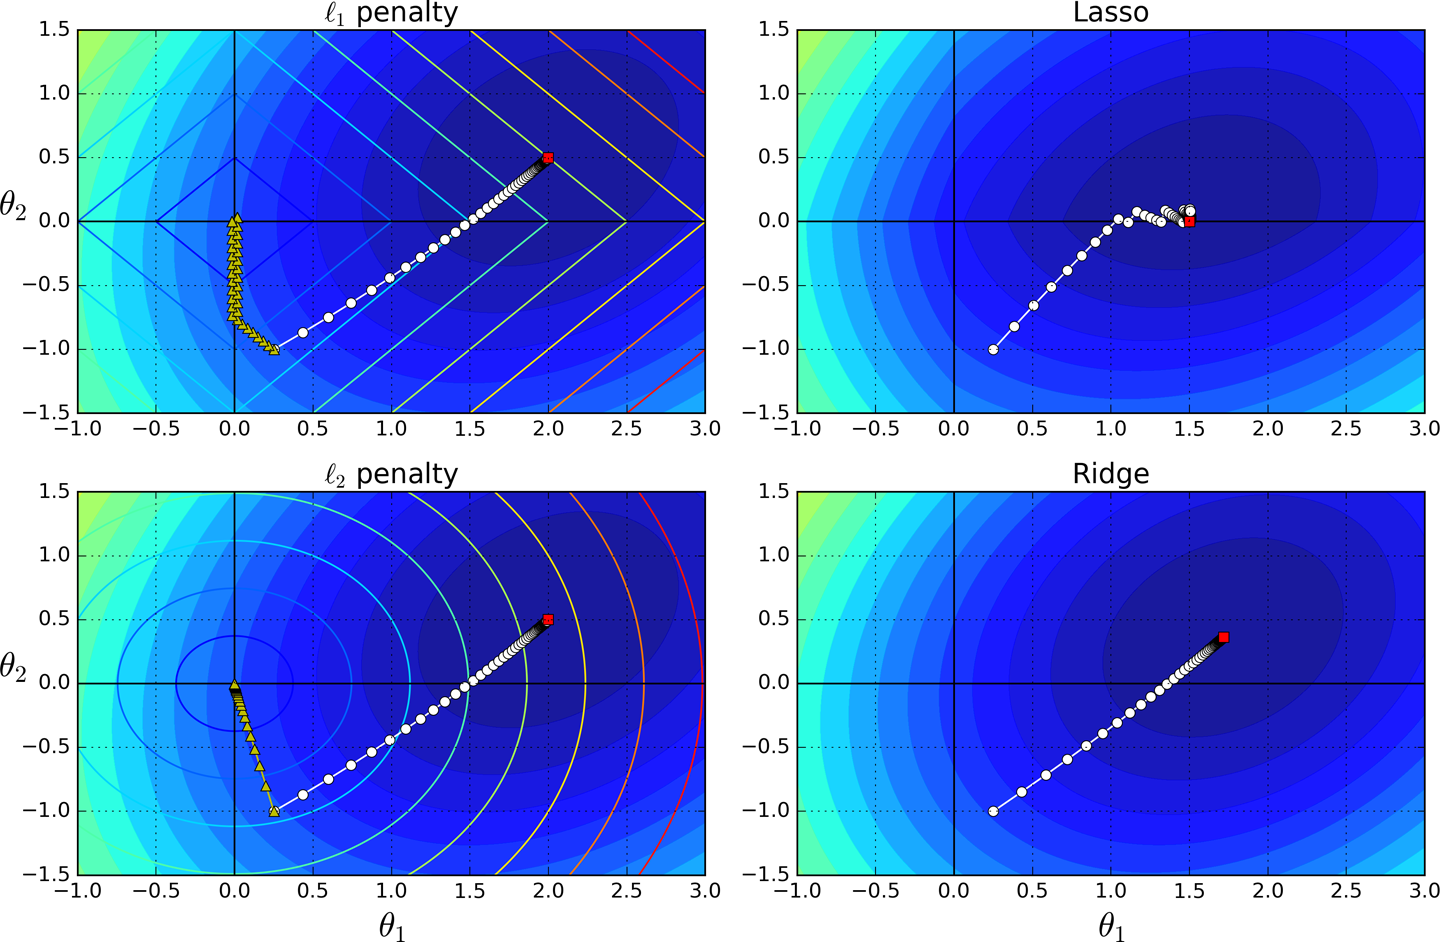
\includegraphics[width=\textwidth]{Figs/section_4/overfitting_loss.png}
    			\caption{Convergence diagram for different losses, \href{https://www.oreilly.com/library/view/hands-on-machine-learning/9781491962282/ch04.html}{Source}}
    		\end{figure}
    	\end{column}
    \end{columns}
\end{frame}
\begin{frame}{L1/L2 Regularization}
    \begin{itemize}
        \item L1/L2 regularizer functions (review)
    \end{itemize}
	\begin{columns}
		\begin{column}[c]{0.5\textwidth}
			\centering
			\begin{equation*}
				\centering
				\mathlarger{\mathlarger{
							L1: R(w) = \vert w\vert
				}}
			\end{equation*}
			\begin{equation*}
				\centering
				\mathlarger{\mathlarger{
							L2: R(w) = w^2
				}}
			\end{equation*}
		\end{column}
		\begin{column}[c]{0.5\textwidth}
			\begin{figure}[H]
				\centering
				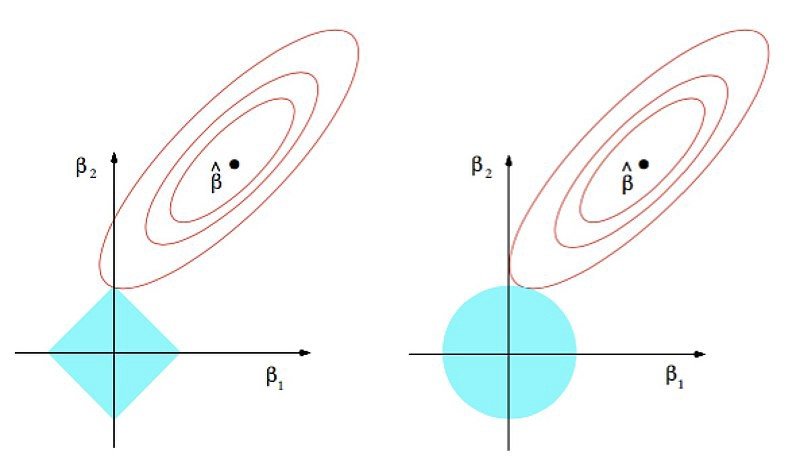
\includegraphics[width=\textwidth]{Figs/section_4/l1l2_reg.jpeg}
				\caption{L1/L2 regularizers' solution diagram, \href{https://towardsdatascience.com/understanding-l1-and-l2-regularization-93918a5ac8d0}{Source}}
			\end{figure}
		\end{column}
	\end{columns}
    
    \begin{itemize}
        \item You can also combine the two different regularizers (Elastic Net).
    \end{itemize}
	\vspace{0.05\textheight}
    \begin{equation*}
        \mathlarger{\mathlarger{
        R(w) = \beta w^2 + \vert w\vert
        }}
    \end{equation*}
\end{frame}

\begin{frame}{Solution 2: Early Stopping}
    \begin{itemize}
        \item Stop the training procedure when the validation error is \tc{keywords}{minimum}.
    \end{itemize}
	\vspace{0.1\textheight}
    \begin{figure}
	\centering
	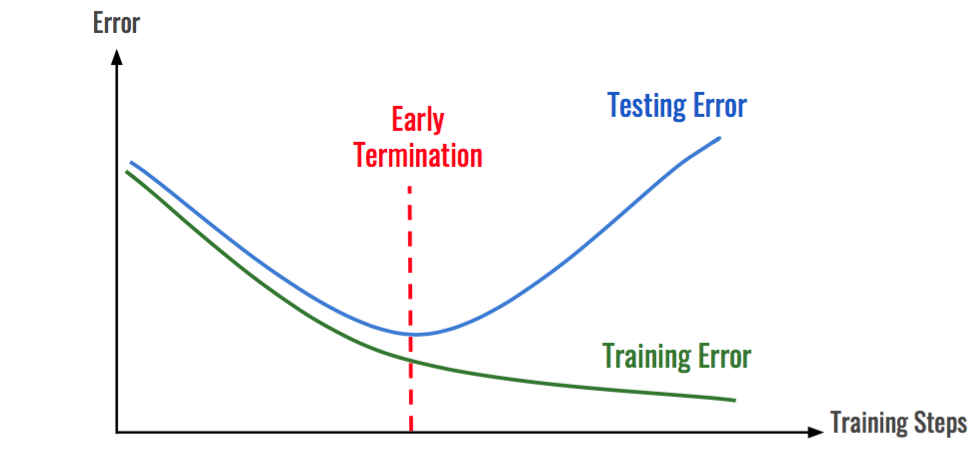
\includegraphics[width=0.8\textwidth]{Figs/Early Stopping.png}
	\caption{Early Stopping diagram, \href{https://medium.com/analytics-v7idhya/early-stopping-with-pytorch-to-restrain-your-model-from-overfitting-dce6de4081c5}{Source}}
    \end{figure}
\end{frame}

\begin{frame}{Dropout: Training Time}
	\begin{itemize}
		\item In each forward pass, \tc{keywords}{randomly} set some neurons to zero.
		\medskip
		\item The probability of dropping out for each neuron, which is called \tc{keywords}{dropout rate}, is a hyperparameter.
		\begin{itemize}
			\item 0.5 is a common dropout rate.
		\end{itemize}
		\medskip
		\item The probability of not dropping out is also called the \tc{keywords}{keep probability}.
	\end{itemize}
	\begin{figure}[H]
		\centering
		\begin{subfigure}[b]{0.45\textwidth}
			\centering
			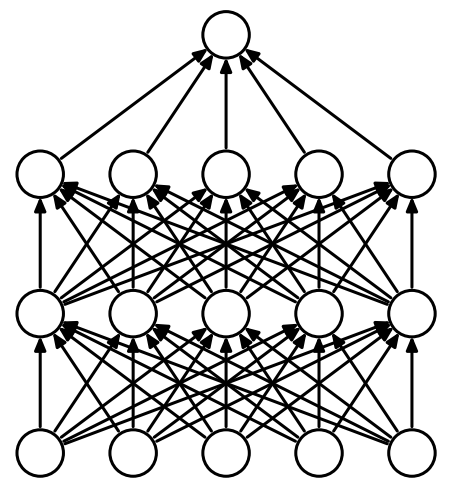
\includegraphics[height=0.4\textheight]{Figs/Dropout-before.png}
		\end{subfigure}
		\begin{subfigure}[b]{0.45\textwidth}
			\centering
			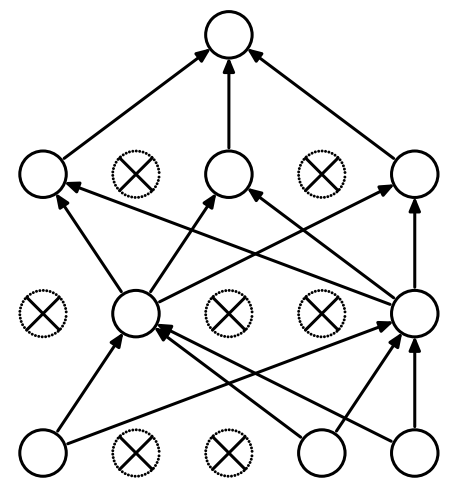
\includegraphics[height=0.4\textheight]{Figs/Dropout-after.png}
		\end{subfigure}
		\caption{Behavior of dropout at training time, \href{https://www.cs.toronto.edu/~hinton/absps/JMLRdropout.pdf}{Source}}
	\end{figure}
\end{frame}
\begin{frame}{Dropout}
	\begin{itemize}
		\item How can this possibly be a good idea?
		\medskip
		\begin{itemize}
			\item It prevents the \tc{keywords}{co-adaptation of features}
		\end{itemize}
	\end{itemize}
	\begin{figure}[H]
		\centering
		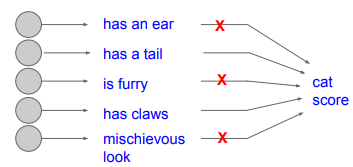
\includegraphics[height=0.4\textheight]{Figs/section_4/dropout_why.png}
		\caption{Discrimination of neurons at training time. \cite{cs231n-2018-lecture7}}
	\end{figure}
\end{frame}
\begin{frame}{Dropout}
	\begin{itemize}
		\item How can this possibly be a good idea?
		\medskip
		\begin{itemize}
			\item It trains a \tc{keywords}{large ensemble of models} that share parameters.
			\medskip
			\item A fully connected layer with 4096 neurons has $2^{4096} \sim 10^{1233}$ possible masks! There are only $10^{82}$ atoms in the universe!
		\end{itemize}
	\end{itemize}
	\begin{figure}[H]
		\centering
		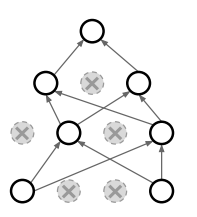
\includegraphics[height=0.4\textheight]{Figs/section_4/dropout_why2.png}
		\caption{Behavior of dropout at training time. \cite{cs231n-2018-lecture7}}
	\end{figure}
\end{frame}
\begin{frame}{Dropout: Test Time}
	\begin{itemize}
		\item Dropout makes our output random at training time.
		\medskip
	\end{itemize}
	\begin{equation*}
		\mathlarger{\mathlarger{
		y = f_W(x, \underbrace{z}_{\text{\tiny{\tc{keywords}{random mask}}}})
	}}
	\end{equation*}
	\begin{itemize}
		\item We want to \tc{keywords}{average out} the randomness at test time,
		\medskip
	\end{itemize}
	\begin{equation*}
		\mathlarger{\mathlarger{
			y = f(x) = E_z[f(x, z)] = \int p(z)f(x, z) dz
		}}
	\end{equation*}
	\begin{itemize}
		\item But this integral seems complicated.
		\medskip
		\item Let's approximate the integral for a superficial layer where dropout rate is 0.5.
	\end{itemize}
\end{frame}
\begin{frame}{Dropout: Test Time}
	\begin{columns}
		\begin{column}{0.5\textwidth}
			\begin{align*}
				E_{train}[a] = \frac{1}{4}(w_1 x + w_2 y)
				+ \frac{1}{4}(w_1 x + 0 y) \\
				+ \frac{1}{4}(0 x + w_2 y) + \frac{1}{4}(0 x + 0 y) \\
				= \frac{1}{2}(w_1 x + w_2 y) \\
				E_{test}[a] = w_1 x + w_2 y \\
				\Rightarrow E_{test}[a] = \underbrace{0.5}_{\text{\tc{keywords}{dropout probability}}} E_{train}[a]
			\end{align*}
		\end{column}
		\begin{column}{0.5\textwidth}
			\begin{figure}[H]
				\centering
				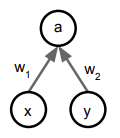
\includegraphics[height=0.4\textheight]{Figs/section_4/dropout_test.png}
				\caption{Simple neural network. \cite{cs231n-2018-lecture7}}
			\end{figure}
		\end{column}
	\end{columns}
\end{frame}

\begin{frame}{Solution: Batch Norm Layer}
	\begin{itemize}
		\item It is used to \tc{keywords}{normalize} the data.
	\end{itemize}
	\begin{figure}[H]
		\centering
		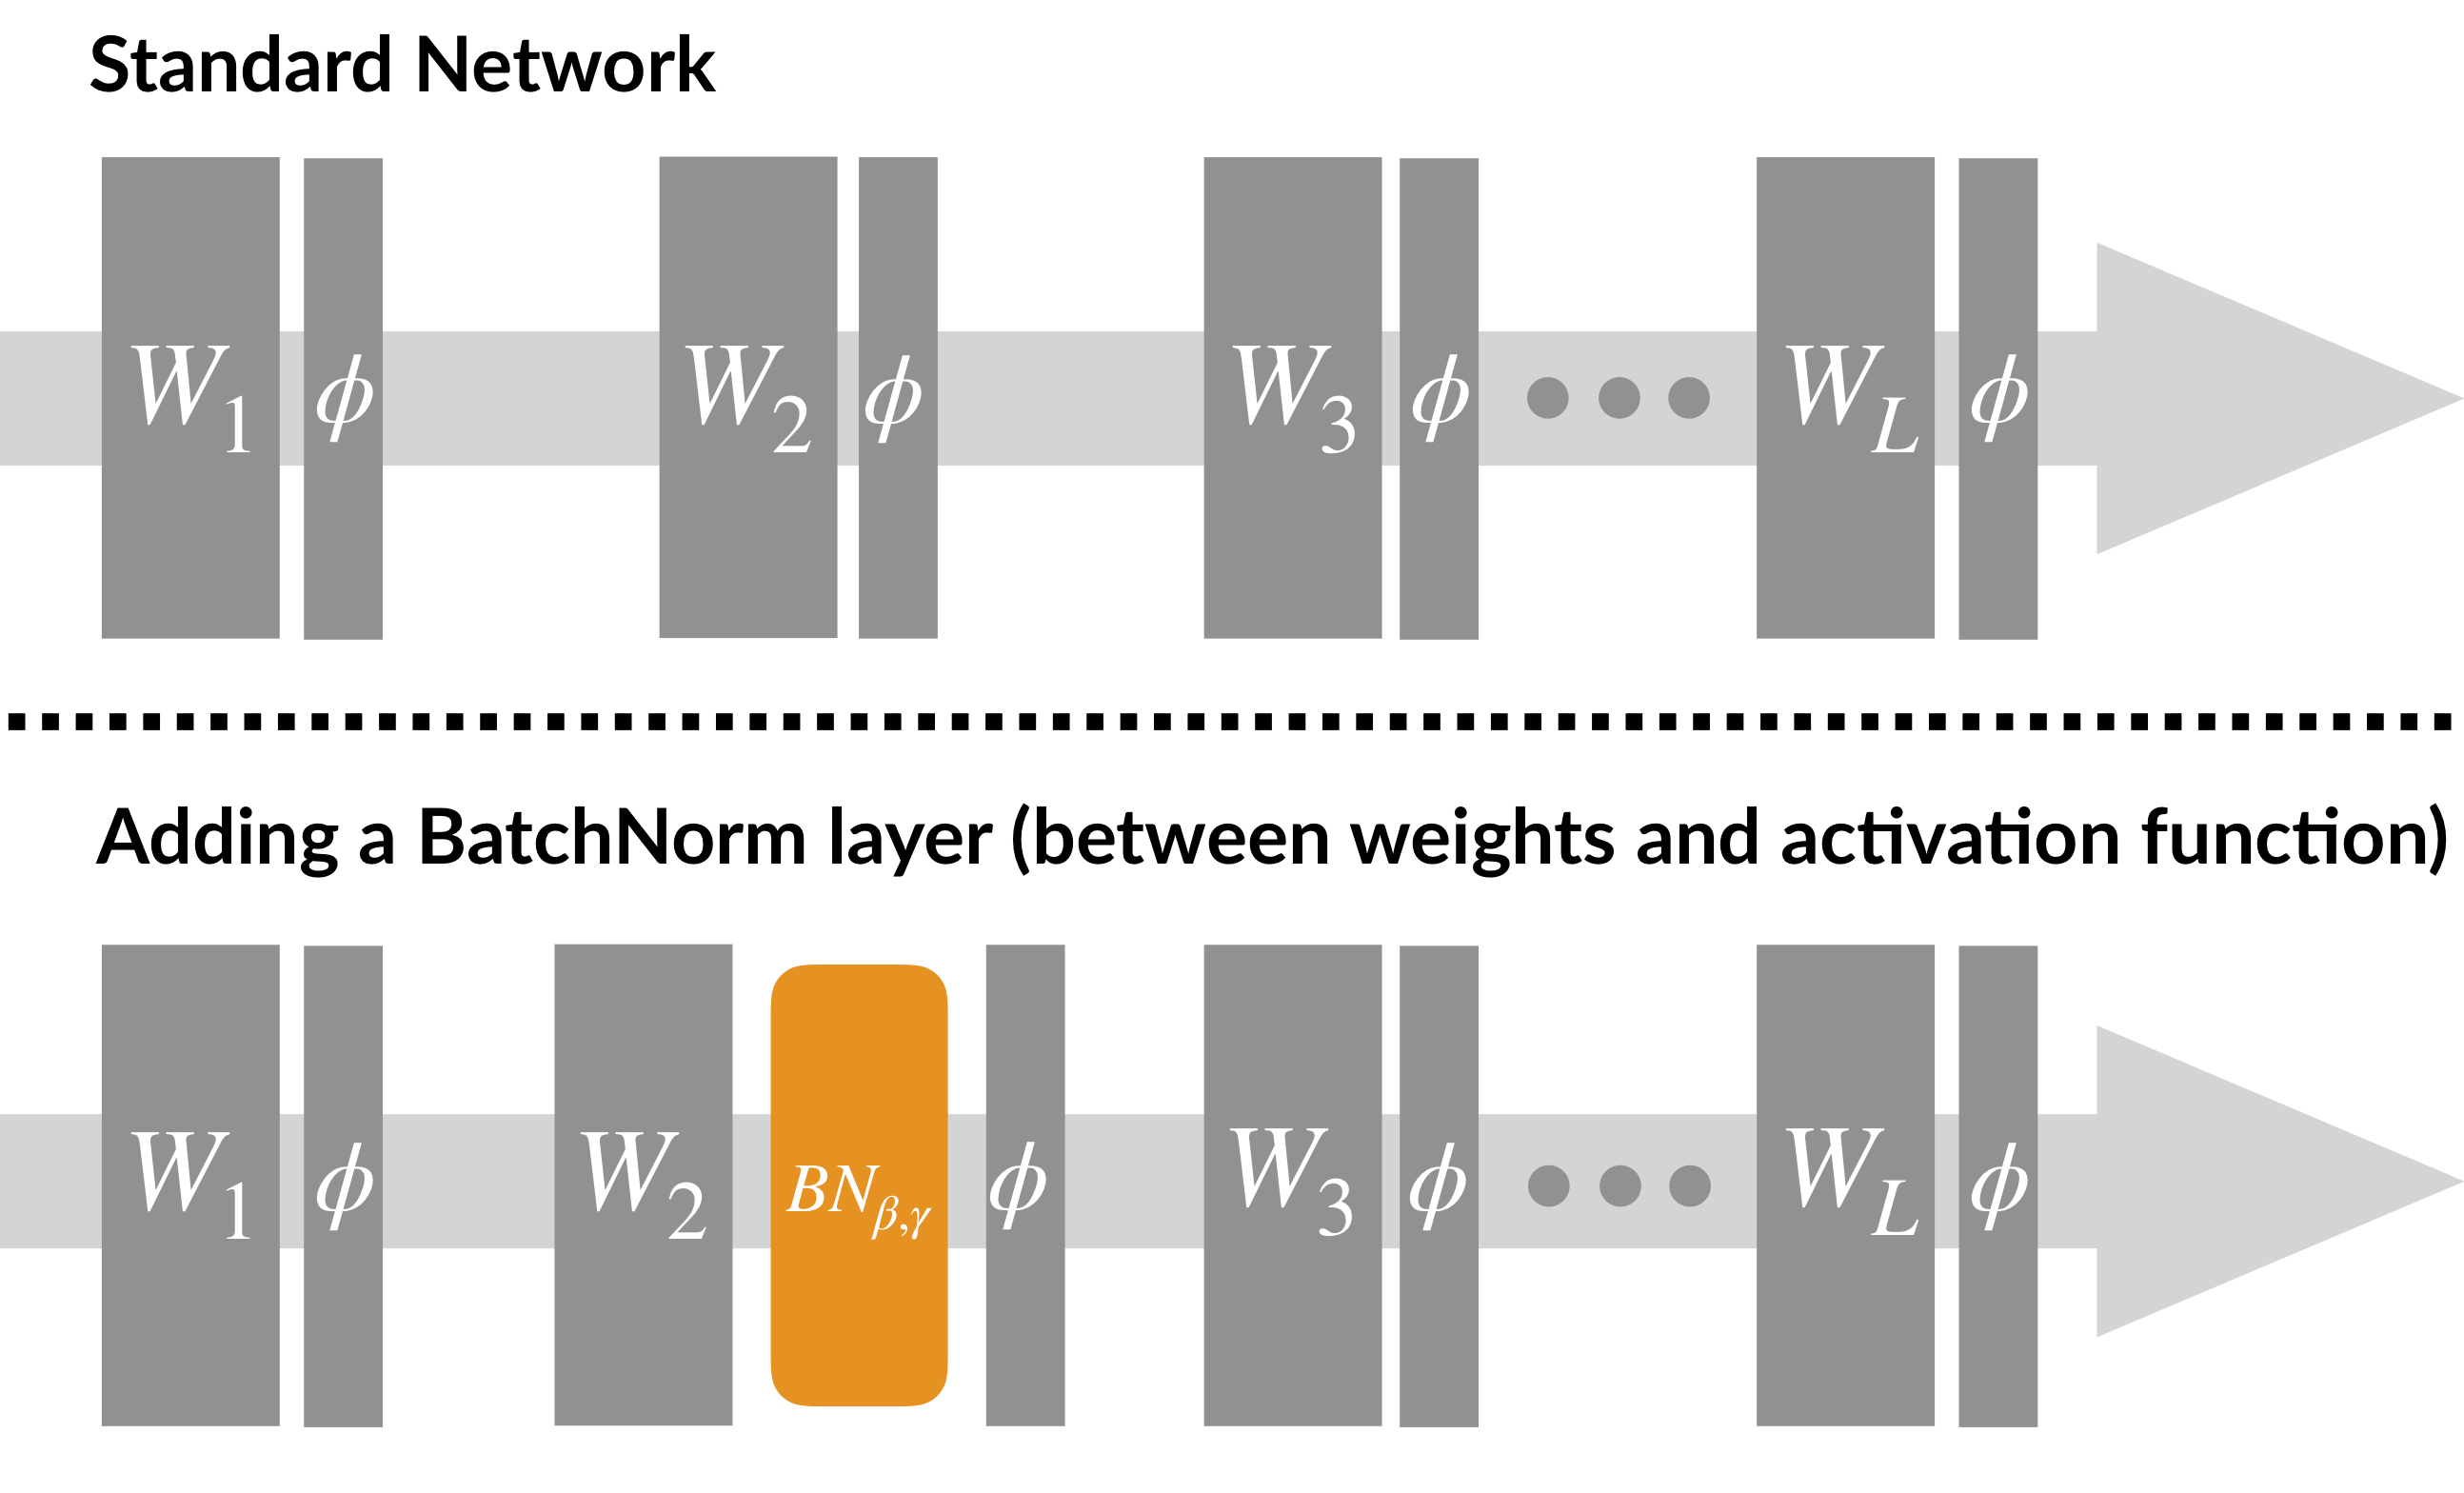
\includegraphics[width=0.75\textwidth]{Figs/section_4/batchnorm_2.jpg}
		\caption{The suggested place to put a BatchNorm layer, \href{https://gradientscience.org/batchnorm/}{Source}}
	\end{figure}
\end{frame}
\begin{frame}{Batch Norm: Training Time}
	\begin{itemize}
		\item First, it zero-centers and normalizes the batch.
	\end{itemize}
	\vspace{0.05\textheight}
	\begin{equation*}
		\mathlarger{
			\mu_B := \frac{1}{N_B} \sum{x_B^{(i)}}
		}
	\end{equation*}
	\begin{equation*}
		\mathlarger{
			\sigma_B^2 := \frac{1}{N_B} \sum{(x_B^{(i)} - \mu_B)^2}
		}
	\end{equation*}
	\begin{equation*}
		\mathlarger{
			\hat{x_B}^{(i)} = \frac{x_B^{(i)} - \mu_B}{\sqrt{\sigma^2_B + \epsilon}}
		}
	\end{equation*}
	\begin{itemize}
		\item Then, scales and shifts the batch with two learnable parameters $\gamma, \beta$.
	\end{itemize}
	\vspace{0.05\textheight}
	\begin{equation*}
		\mathlarger{
			y_B^{(i)} = \gamma \hat{x_B}^{(i)} + \beta	
		}
	\end{equation*}
\end{frame}
\begin{frame}{Batch Norm: Test Time}
	\begin{itemize}
		\item To zero-center and normalize the input, we need the average and variance of the whole data.
		\medskip
		\item Those parameters can be acquired during the training.
		\medskip
		\item Therefore, we need two more trainable parameters.
	\end{itemize}
	\vspace{0.1\textheight}
		\begin{equation*}
			\mathlarger{
				\mu_D := \frac{1}{N} \sum{x^{(i)}}
			}
		\end{equation*}
		\begin{equation*}
			\mathlarger{
				\sigma_D^2 := \frac{1}{N} \sum{(x^{(i)} - \mu)^2}
			}
		\end{equation*}
\end{frame}
\begin{frame}{Batch Norm: Performance}
	\begin{itemize}
		\item Normalizing the data improves the convergence speed by a considerable amount.
	\end{itemize}
	\begin{figure}[H]
		\centering
		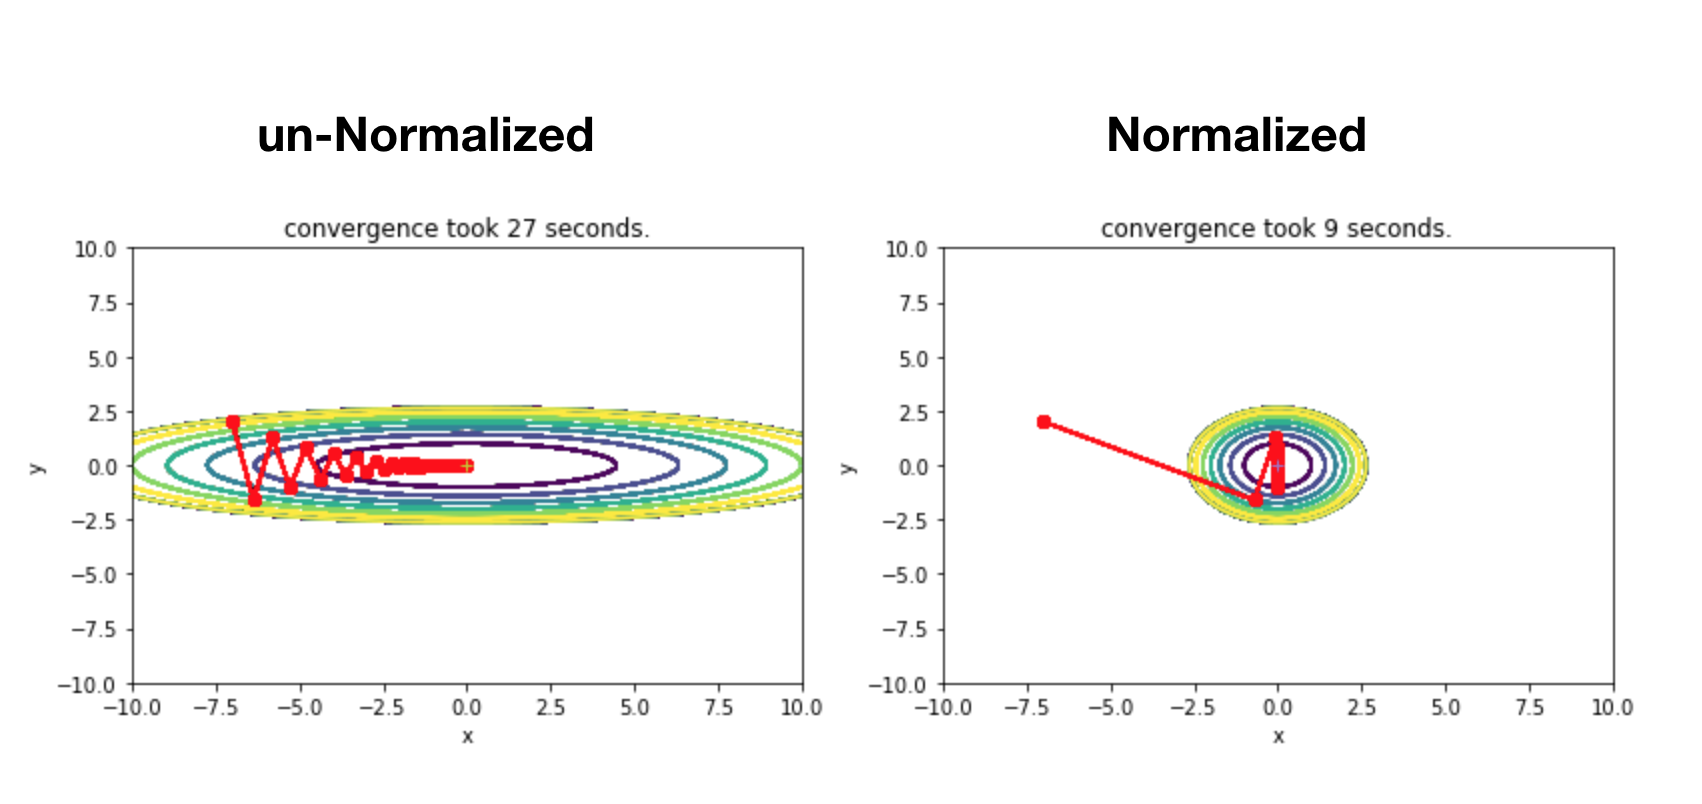
\includegraphics[width=0.8\textwidth]{Figs/section_4/batchnorm_3.png}
		\caption{BatchNorm performance. Convergence speed is increased by 200\%,  \href{https://jsideas.net/batch_normalization/}{Source}}
	\end{figure}
\end{frame}
\begin{frame}{Batch Norm: Pros}
	\begin{itemize}
		\item Vanishing/Exploding gradient problem is reduced by a considerable amount.
		\medskip
%			\begin{itemize}
			\item You can use even saturating activation functions.
			\medskip
			\item The network is much less sensitive to the initial weight.
			\medskip
			\item We're able to use larger learning rates, which speeds up the training.
%			\end{itemize}
		\medskip
		\item It also acts as a regularizer.
		\medskip
		\begin{itemize}
			\item There is no need for other regularizer techniques.
		\end{itemize}
	\end{itemize}
\end{frame}
\begin{frame}{Batch Norm: Cons}
	\begin{itemize}
		\item It increases model parameters and prediction latency.
		\medskip
		\begin{itemize}
			\item Solution: after the training procedure, we can mix the BatchNorm layer with its previous layer to hold the prediction latency.
		\end{itemize}
	\end{itemize}
	\begin{columns}
		\begin{column}[c]{0.45\textwidth}
			\centering
			\begin{equation*}
				\mathlarger{x'^{(i)} = W x^{(i)} + b}
			\end{equation*}
			\begin{equation*}
				\mathlarger{y^{(i)} = \frac{x'^{(i)} - \mu}{\sqrt{\sigma^2 + \epsilon}} + \beta}
			\end{equation*}
		\end{column}
		\begin{column}[c]{0.1\textwidth}
			\centering
			\begin{equation*}
				\mathlarger{\mathlarger{
				\Rightarrow
			}}
			\end{equation*}
		\end{column}
		\begin{column}[c]{0.45\textwidth}
			\centering
			\begin{equation*}
				\mathlarger{y^{(i)} = W' x^{(i)} + b'}
			\end{equation*}
			\begin{equation*}
				\mathlarger{
					W' := \frac{1}{\sqrt{\sigma^2 + \epsilon}} W	
				}
			\end{equation*}
			\begin{equation*}
				\mathlarger{
					b' := \beta + \frac{b- \mu}{\sqrt{\sigma^2 + \epsilon}}	
				}
			\end{equation*}
		\end{column}
	\end{columns}
	\begin{itemize}
		\item Where $\mu$ and $\sigma$ are the mean and variance for the test time.
	\end{itemize}
\end{frame}